\documentclass[11pt,a4paper,center,notitlepage]{article}
\usepackage[backend=biber]{biblatex}

% Use Natbib reference style
%\usepackage{natbib}
 %\bibliographystyle{abbrvnat}

%\usepackage[backend=biber,style=authoryear,natbib=true]{biblatex} % Use the bibtex backend with the authoryear citation style (which resembles APA)

%\addbibresource{mybib.bib} % The filename of the bibliography
% For tabular
\usepackage{tabularx}
%\usepackage{arydshln,leftidx,mathtools}
%
%\setlength{\dashlinedash}{.4pt}
%\setlength{\dashlinegap}{.8pt}

\usepackage[autostyle=true]{csquotes} % Required to generate language-dependent quotes in the bibliography

\usepackage{algorithm}
\usepackage{algpseudocode}
\usepackage[utf8]{inputenc} 
%\usepackage[T1]{fontenc}
\usepackage[english]{babel} 
\usepackage{color}
\usepackage{textcomp,multicol,enumerate,amsmath,amssymb,amsthm,eufrak,latexsym,makeidx}
\newcommand{\vertiii}[1]{{\left\vert\kern-0.25ex\left\vert\kern-0.25ex\left\vert #1 
    \right\vert\kern-0.25ex\right\vert\kern-0.25ex\right\vert}}
% For insert figure
\usepackage{subfig}
\usepackage{graphicx,epstopdf}

%% Color Reference
\usepackage[usenames,dvipsnames,svgnames,table]{xcolor}
\usepackage[colorlinks=true,
            linkcolor=blue,
            urlcolor=gray,
            citecolor=magenta]{hyperref}
            
\allowdisplaybreaks
% No page break in Bibliography
\numberwithin{equation}{section}
\addto{\captionsenglish}{%
  \renewcommand{\bibname}{References}
}


\textwidth=16 cm
\textheight=22 cm
\topmargin= -1 cm
\oddsidemargin=0 cm
\evensidemargin=1 cm
\parindent=0.6 cm
\parskip=1.5 mm
\newtheorem{lemma}{Lemma}[section]
\newtheorem{corollary}{Corollary}[section]
\newtheorem{definition}{Definition}[section]
\newtheorem{prop}{Proposition}[section]
\newtheorem{theorem}{Theorem}[section]
\newtheorem{prob}{Problem}[section]
\newtheorem{notation}{Notation}[section]
\newtheorem{remark}{Remark}[section]
\newtheorem{example}{Example}[section]
\newtheorem{ques}{Question}[section]
\newtheorem{sol}{Solution}[section]
\renewcommand{\thenotation}{}
\renewcommand{\thesection}{\arabic{section}}
\renewcommand{\thesubsection}
{\arabic{section}.\arabic{subsection}}
\pagestyle{plain}

% Reference
\newcommand{\er}{\eqref}

%\newtheorem{theorem}{Theorem}[section]
%\newtheorem{corollary}[theorem]{Corollary}
%\newtheorem{lemma}[theorem]{Lemma}
%\newtheorem{proposition}[theorem]{Proposition}

%\theoremstyle{definition}
%\newtheorem{definition}[theorem]{Definition}
%\newtheorem{remark}{Remark}
%\newtheorem{properties}{Properties}
%\newtheorem*{notation}{Notation}
%\newtheorem{counter}{Counter-example}
%\newtheorem{open}{Open problem}
%\newtheorem{conjecture}{Conjecture}


%% FONT commands
\newcommand{\txt}[1]{\;\text{ #1 }\;}%% Used in math only
\newcommand{\tbf}{\textbf}%% Bold face. Usage: \tbf{...}
\newcommand{\tit}{\textit}%% Italic
\newcommand{\tsc}{\textsc}%% Small caps
\newcommand{\trm}{\textrm}
\newcommand{\mbf}{\mathbf}%% Math bold
\newcommand{\mrm}{\mathrm}%% Math Roman
\newcommand{\bsym}{\boldsymbol}%% Bold math symbol
%%Macros for changing font size in math.
\newcommand{\scs}{\scriptstyle}%% as in subscript
\newcommand{\sss}{\scriptscriptstyle}%% as in sub-subscript
\newcommand{\txts}{\textstyle}
\newcommand{\dsps}{\displaystyle}
%%Macros for changing font size in text.
\newcommand{\fnz}{\footnotesize}
\newcommand{\scz}{\scriptsize}
%%\tiny<\scz<\fsz<\small<\large<\Large<\huge<\Huge
%%%%%%%%%%%%
%%%%%%%%%%%%
%% EQUATION commands
\newcommand{\be}{\begin{equation}}
\newcommand{\bel}[1]{\begin{equation}\label{#1}}
\newcommand{\ee}{\end{equation}}
%% This macro does not work with amstex.
\newcommand{\eqnl}[2]{\begin{equation}\label{#1}{#2}\end{equation}}
%%use not advisable; confusing
\newcommand{\barr}{\begin{eqnarray}}
\newcommand{\earr}{\end{eqnarray}}
\newcommand{\bars}{\begin{eqnarray*}}
\newcommand{\ears}{\end{eqnarray*}}
\newcommand{\nnu}{\nonumber \\}
%%%%%%%%%%%%%%%
%% Unnumbered THEOREM env.
%% New env. to be used for unnumbered theorem, lemma etc.
%%(but with specified name)

\newtheorem{subn}{\name}
\renewcommand{\thesubn}{}
\newcommand{\bsn}[1]{\def\name{#1}\begin{subn}}
\newcommand{\esn}{\end{subn}}
%%%%%%%%%%%%%%
%% NUMBERED THEOREM env.
%% Environments: theorem, lemma, corollary defintion and
%%related commands,
%% designed to provide consecutive numbering of these forms.


\newtheorem{sub}{\name}[section]
\newcommand{\dn}[1]{\def\name{#1}}

%%used in conjuction with sub or subn.

\newcommand{\bs}{\begin{sub}}
\newcommand{\es}{\end{sub}}
\newcommand{\bsl}[1]{\begin{sub}\label{#1}}
	
%% the above must be preceeded by \dn (name definition),
%% however this is superceded by the list of commands bth etc. below.
%%%%%%%%%%%%
%% NUMBERED THEOREM env. (cont.)
%% List of commands derived from 'sub' env. for theorem, lemma etc.
%% designed to provide consecutive numbering of these forms.
\newcommand{\bth}[1]{\def\name{Theorem}\begin{sub}\label{t:#1}}
\newcommand{\blemma}[1]{\def\name{Lemma}\begin{sub}\label{l:#1}}
\newcommand{\bcor}[1]{\def\name{Corollary}\begin{sub}\label{c:#1}}	
\newcommand{\bdef}[1]{\def\name{Definition}\begin{sub}\label{d:#1}}
\newcommand{\bprop}[1]{\def\name{Proposition}\begin{sub}\label{p:#1}}	
%% ARRAY commands.%%%%%%%%%%%%%%%%%%%%%%%%%%%%%%%%%%
%% RERERENCE commands.
%% \newcommand{\R}[1]{(\ref{#1})}

\newcommand{\R}{\eqref}
\newcommand{\re}{\eqref}
\newcommand{\rth}[1]{Theorem~\ref{t:#1}}
\newcommand{\rlemma}[1]{Lemma~\ref{l:#1}}
\newcommand{\rcor}[1]{Corollary~\ref{c:#1}}
\newcommand{\rdef}[1]{Definition~\ref{d:#1}}
\newcommand{\rprop}[1]{Proposition~\ref{p:#1}}
%%%%%%%%%%%
\newcommand{\BA}{\begin{array}}
\newcommand{\EA}{\end{array}}
\newcommand{\BAN}{\renewcommand{\arraystretch}{1.2}
\setlength{\arraycolsep}{2pt}\begin{array}}
\newcommand{\BAV}[2]{\renewcommand{\arraystretch}{#1}
\setlength{\arraycolsep}{#2}\begin{array}}
%Note: The first variable gives the amount of stretching:
%(#1) x default.
%For instance #1=1.2 means a 20% stretching.
%The second variable should be
%written for instance in the form  4pt ; here the default is 5pt
%\newcommand{\EAN}{\end{array}\setlength{\arraycolsep}{5pt}}
\newcommand{\BSA}{\begin{subarray}}
\newcommand{\ESA}{\end{subarray}}	
%Note: These are used in subscripts as well as superscripts.
%They work essentially like 'array'.

\newcommand{\BAL}{\begin{aligned}}
	\newcommand{\EAL}{\end{aligned}}
\newcommand{\BALG}{\begin{alignat}}
	\newcommand{\EALG}{\end{alignat}}
%% the abbrev. does not work with latex2e
\newcommand{\BALGN}{\begin{alignat*}}
	\newcommand{\EALGN}{\end{alignat*}}
%% the abbrev. does not work with latex2e
%% The 'aligned' environment must be placed inside an 'equation' env.
%% in the same way as the array.
%% One could use also the 'align' env. or the 'alignat' env.
%% However in this case each line is numbered, unless '\notag' is used.
%% The 'alignat'
%% has a slightly different format (the number of columns must be %%specified in advance)
%% but it has the advantage that the distance between columns
%%is at our disposition.
%% (The default would be zero distance.) Using 'alignat*' we can have %%the advantages
%% of alignat plus the situation where separate lines are not numbered.
%% However in this case there is no numbering at all
%%(unless we provide a tag).
%%%%%%%%%%
%% PROOF, REMARK etc.
\newcommand{\note}[1]{\noindent\textit{#1.}\hspace{2mm}}
\newcommand{\Proof}{\note{Proof}}
%\newcommand{\qed}{\hspace{10mm}\hfill $\square$}
%\newcommand{\qed}{\\${}$ \hfill $\square$}
\newcommand{\Remark}{\note{Remark}}
%%%%%%%% Style command.
\newcommand{\modin}{$\,$\\[-4mm] \indent}
%% To be used after \section in order to start new line with \indent.
%%%%%%%%%%%%
%% MATHEMATICAL symbols
\newcommand{\forevery}{\quad \forall}
\newcommand{\set}[1]{\{#1\}}
\newcommand{\setdef}[2]{\{\,#1:\,#2\,\}}
\newcommand{\setm}[2]{\{\,#1\mid #2\,\}}
%% Arrows
\newcommand{\mt}{\mapsto}
\newcommand{\lra}{\longrightarrow}
\newcommand{\lla}{\longleftarrow}
\newcommand{\llra}{\longleftrightarrow}
\newcommand{\Lra}{\Longrightarrow}
\newcommand{\Lla}{\Longleftarrow}
\newcommand{\Llra}{\Longleftrightarrow}
\newcommand{\warrow}{\rightharpoonup}

%% Brackets, delimiters
\newcommand{\paran}[1]{\left (#1 \right )}
%% adjustable parantheses
\newcommand{\sqbr}[1]{\left [#1 \right ]}
%% adjustable square brackets
\newcommand{\curlybr}[1]{\left \{#1 \right \}}
%% adjustable curly brackets
\newcommand{\abs}[1]{\left |#1\right |}

%% adjustable vertical delimiters
\newcommand{\norm}[1]{\left \|#1\right \|}

%% adjustable norm
\newcommand{\paranb}[1]{\big (#1 \big )}

%% non-adjustable parantheses (big)
\newcommand{\lsqbrb}[1]{\big [#1 \big ]}

%% non-adjustable square brackets (big)
\newcommand{\lcurlybrb}[1]{\big \{#1 \big \}}

%% non-adjustable curly brackets(big)
\newcommand{\absb}[1]{\big |#1\big |}

%% non-adjustable vertical delimiters(big)
\newcommand{\normb}[1]{\big \|#1\big \|}

%% non-adjustable norm (big)
\newcommand{	\paranB}[1]{\Big (#1 \Big )}

%% non-adjustable parantheses (Big)
\newcommand{\absB}[1]{\Big |#1\Big |}

%% non-adjustable vertical delimiters(Big)
\newcommand{\normB}[1]{\Big \|#1\Big \|}%% non-adjustable norm (Big)
\newcommand{\produal}[1]{\langle #1 \rangle}%% the pairing of X' and X
%%%%%%%%%%%%%%%%%
%% Adjustable parantheses etc. in a different DEFINITION format.
%\def\adp(#1){\left (#1 \right )}%% adjustable parantheses
%\def\adsb(#1){\left [#1\right ]}%% adjustable square brackets
%\def\adcb(#1){\left \{#1\right \}}%% adjustable curly brackets
%\def\abs|#1|{\left |#1\right |}%% adjustable vertical delimiters
%%%%%%%%%%%%%%%%
%% More mathematical symbols
\newcommand{\thkl}{\rule[-.5mm]{.3mm}{3mm}}
\newcommand{\thknorm}[1]{\thkl #1 \thkl\,}
\newcommand{\trinorm}[1]{|\!|\!| #1 |\!|\!|\,}
\newcommand{\bang}[1]{\langle #1 \rangle}%% angle bracket
\def\angb<#1>{\langle #1 \rangle}%% angle bracket
%% The two last lines yield the same result.
%% The second is used as follows: \angb<a,b>
\newcommand{\vstrut}[1]{\rule{0mm}{#1}}
\newcommand{\rec}[1]{\frac{1}{#1}}
%% OPERATOR names.
%% OPERATOR names.
\newcommand{\opname}[1]{\mbox{\rm #1}\,}
\newcommand{\supp}{\opname{supp}}
\newcommand{\dist}{\opname{dist}}
\newcommand{\myfrac}[2]{{\displaystyle \frac{#1}{#2} }}
\newcommand{\myint}[2]{{\displaystyle \int_{#1}^{#2}}}
\newcommand{\mysum}[2]{{\displaystyle \sum_{#1}^{#2}}}
\newcommand {\dint}{{\displaystyle \myint\!\!\myint}}%%%%%%%%%%
%%%%%%% SPACE commands
\newcommand{\q}{\quad}
\newcommand{\qq}{\qquad}
\newcommand{\hsp}[1]{\hspace{#1mm}}
\newcommand{\vsp}[1]{\vspace{#1mm}}
%%%%%%%%%%%
%% ABREVIATIONS
\newcommand{\ity}{\infty}
\newcommand{\prt}{\partial}
\newcommand{\sms}{\setminus}
\newcommand{\ems}{\emptyset}
\newcommand{\ti}{\times}
\newcommand{\pr}{^\prime}
\newcommand{\ppr}{^{\prime\prime}}
\newcommand{\tl}{\tilde}
\newcommand{\sbs}{\subset}
\newcommand{\sbeq}{\subseteq}
\newcommand{\nind}{\noindent}
\newcommand{\ind}{\indent}
\newcommand{\ovl}{\overline}
\newcommand{\unl}{\underline}
\newcommand{\nin}{\not\in}
\newcommand{\pfrac}[2]{\genfrac{(}{)}{}{}{#1}{#2}}

%% frac with parantheses.
%%%%%%%%%%%
%%%%%%%%%%%%%

%%Macros for Greek letters.
\def\ga{\alpha}     \def\gb{\beta}       \def\gg{\gamma}
\def\gc{\chi}       \def\gd{\delta}      \def\gep{\epsilon}
\def\gth{\theta}                         \def\vge{\varepsilon}
\def\gf{\varphi}       \def\vgf{\varphi}    \def\gh{\eta}
\def\gi{\iota}      \def\gk{\kappa}      \def\gl{\lambda}
\def\gm{\mu}        \def\gn{\nu}         \def\gp{\pi}
\def\vgp{\varpi}    \def\gr{\gd}        \def\vgr{\varrho}
\def\gs{\sigma}     \def\vgs{\varsigma}  \def\gt{\tau}
\def\gu{\upsilon}   \def\gv{\vartheta}   \def\gw{\omega}
\def\gx{\xi}        \def\gy{\psi}        \def\gz{\zeta}
\def\Gg{\Gamma}     \def\Gd{\Delta}      \def\Gf{\Phi}
\def\Gth{\Theta}
\def\Gl{\Lambda}    \def\Gs{\Sigma}      \def\Gp{\Pi}
\def\Gw{\Omega}     \def\Gx{\Xi}         \def\Gy{\Psi}

%%Macros for calligraphic letters.
\def\CS{{\mathcal S}}   \def\CM{{\mathcal M}}   \def\CN{{\mathcal N}}
\def\CR{{\mathcal R}}   \def\CO{{\mathcal O}}   \def\CP{{\mathcal P}}
\def\CA{{\mathcal A}}   \def\CB{{\mathcal B}}   \def\CC{{\mathcal C}}
\def\CD{{\mathcal D}}   \def\CE{{\mathcal E}}   \def\CF{{\mathcal F}}
\def\CG{{\mathcal G}}   \def\CH{{\mathcal H}}   \def\CI{{\mathcal I}}
\def\CJ{{\mathcal J}}   \def\CK{{\mathcal K}}   \def\CL{{\mathcal L}}
\def\CT{{\mathcal T}}   \def\CU{{\mathcal U}}   \def\CV{{\mathcal V}}
\def\CZ{{\mathcal Z}}   \def\CX{{\mathcal X}}   \def\CY{{\mathcal Y}}
\def\CW{{\mathcal W}} \def\CQ{{\mathcal Q}}
%%%%%
%%Macros for 'blackboard' letters (See (27) for display.)
\def\BBA {\mathbb A}   \def\BBb {\mathbb B}    \def\BBC {\mathbb C}
\def\BBD {\mathbb D}   \def\BBE {\mathbb E}    \def\BBF {\mathbb F}
\def\BBG {\mathbb G}   \def\BBH {\mathbb H}    \def\BBI {\mathbb I}
\def\BBJ {\mathbb J}   \def\BBK {\mathbb K}    \def\BBL {\mathbb L}
\def\BBM {\mathbb M}   \def\BBN {\mathbb N}    \def\BBO {\mathbb O}
\def\BBP {\mathbb P}   \def\BBR {\mathbb R}    \def\BBS {\mathbb S}
\def\BBT {\mathbb T}   \def\BBU {\mathbb U}    \def\BBV {\mathbb V}
\def\BBW {\mathbb W}   \def\BBX {\mathbb X}    \def\BBY {\mathbb Y}
\def\BBZ {\mathbb Z}

%%Macros for Ghotic (Fraktur) letters.
\def\GTA {\mathfrak A}   \def\GTB {\mathfrak B}    \def\GTC {\mathfrak C}
\def\GTD {\mathfrak D}   \def\GTE {\mathfrak E}    \def\GTF {\mathfrak F}
\def\GTG {\mathfrak G}   \def\GTH {\mathfrak H}    \def\GTI {\mathfrak I}
\def\GTJ {\mathfrak J}   \def\GTK {\mathfrak K}    \def\GTL {\mathfrak L}
\def\GTM {\mathfrak M}   \def\GTN {\mathfrak N}    \def\GTO {\mathfrak O}
\def\GTP {\mathfrak P}   \def\GTR {\mathfrak R}    \def\GTS {\mathfrak S}
\def\GTT {\mathfrak T}   \def\GTU {\mathfrak U}    \def\GTV {\mathfrak V}
\def\GTW {\mathfrak W}   \def\GTX {\mathfrak X}    \def\GTY {\mathfrak Y}
\def\GTZ {\mathfrak Z}   \def\GTQ {\mathfrak Q}
\def\sign{\mathrm{sign\,}}
\def\bdw{\prt\Gw\xspace}
\def\nabu{|\nabla u|}
\def\tr{\mathrm{tr\,}}
\def\gap{{\ga_+}}
\def\gan{{\ga_-}}

\def\N{\mathbb{N}}
\def\Z{\mathbb{Z}}
\def\Q{\mathbb{Q}}
\def\R{\mathbb{R}}


\def\Proof.{{\bf{Proof. }}}
\def\End{\hspace{1cm} $\Box$\\}


\renewcommand{\baselinestretch}{1.1}

\let\e=\varepsilon
\let\vp=\varphi
\let\t=\tilde
\let\ol=\overline
\let\ul=\underline
\let\.=\cdot
\let\0=\emptyset
\let\mc=\mathcal
\def\ex{\exists\;}
\def\fa{\forall\;}
\def\se{\ \Leftarrow\ }
\def\solose{\ \Rightarrow\ }
\def\sse{\ \Leftrightarrow\ }
\def\meno{\,\backslash\,}
\def\pp{,\dots,}
\def\D{\mc{D}}
\def\O{\Omega}


\def\loc{\text{\rm loc}}
\def\diam{\text{\rm diam}}
\def\dist{\text{\rm dist}}
\def\dv{\text{\rm div}}
\def\sign{\text{\rm sign}}
\def\supp{\text{\rm supp}}
\def\tr{\text{\rm Tr}}
\def\vec{\text{\rm vec}}
\def\inter{\text{\rm int\,}}
\def\norma#1{\|#1\|_\infty}

\newcommand{\esssup}{\mathop{\rm ess{\,}sup}}
\newcommand{\essinf}{\mathop{\rm ess{\,}inf}}
\newcommand{\su}[2]{\genfrac{}{}{0pt}{}{#1}{#2}}

\def\eq#1{{\rm(\ref{eq:#1})}}
\def\thm#1{Theorem \ref{thm:#1}}
\def\seq#1{(#1_n)_{n\in\N}}
\def\limn{\lim_{n\to\infty}}


\def\PP{\mc{P}}
\def\pe{principal eigenvalue}
\def\MP{maximum principle}
\def\SMP{strong maximum principle}
\def\l{\lambda_1}

\def\bq{\begin{equation}}
\def\eq{\end{equation}}

\def\l{\label}

\newenvironment{formula}[1]{\begin{equation}\label{eq:#1}}	{\end{equation}\noindent}

\title{Notes $\star$ Analyse Num\'erique - Part II: Implementation of the Finite Elements $\star$ Automatic Meshes for Polygonal Structures}
\author{Nguyen Quan Ba Hong\footnote{Master 2 student at UFR math\'ematiques, Universit\'e de Rennes 1, Beaulieu - B\^atiment 22 et 23, 263 avenue du G\'en\'eral Leclerc, 35042 Rennes CEDEX, France.\newline
E-mail: \texttt{nguyenquanbahong@gmail.com} \newline
Blog: \texttt{\url{www.nguyenquanbahong.com}} \newline 
Copyright \copyright\ 2016-2018 by Nguyen Quan Ba Hong. This document may be copied freely for the purposes of education and non-commercial research. Visit my site to get more.}}
\begin{document}
\maketitle
\begin{abstract}
This context includes the material given by Prof. \'Eric Darrigrand in the course \textit{Finite Element Method}, which is taught by Prof. Nicolas Seguin and Prof. \'Eric Darrigrand  in the Master 2 Fundamental Mathematics program 2018-2019, with my \textsc{Matlab} scripts provided.
\end{abstract}
%\textbf{Mathematics Subject Classification (2010):} 
%
%\noindent
%\textbf{Keywords:} \emph{}
\maketitle
\textbf{Brief introduction.} ``This lecture is a numerical counterpart to \textit{Sobolev spaces \& elliptic equations}. In the first part, after some reminders on linear elliptic partial differential equations, the approximation of the associated solutions by the finite element methods is investigated. Their construction and their analysis are described in one and two dimensions. The second part of the lectures consists in defining a generic strategy for the implementation of the method based on the variational formulation. A program is written in \textsc{Matlab} (implementable with \textsc{Matlab} or \textsc{Octave}).''
\newpage
\tableofcontents
\newpage

\section{Structure of a Mesh}
A mesh of triangles will be represented by two tables: 
\begin{itemize}
\item the table of coordinates of the points, of size $NbPoints \times 2$ (i.e., Number of Points$\times 2$)
\begin{align}
\mbox{coords}\left(l,L\right) = L^e \mbox{ coordinate of the point number }l.
\end{align}
\item the table of triangles, of size $NbTriangles \times NbNodes$ (i.e., Number of Triangles$\times$Number of Nodes)
\begin{align}
\mbox{triangles}\left(k,i\right) = \mbox{number of the }i^{\rm th} \mbox{ node of the triangle number } k.
\end{align}
\end{itemize}
For triangles $\mathbb{P}_1$, $NbNodes =3$; for triangles $\mathbb{P}_2$, $NbNodes =6$.

In \textsc{Matlab}, we use the structure of data \texttt{struct}, similar to the concept of objects of an object-oriented language like C++. We use the following constructor
\begin{verbatim}
function mesh_s = mesh_new(name, coords, triangles)
% define a new mesh_structure
% Author: G. Vial
% Date: 08/09/2010
% Last update: 22/09/11 -- E. Darrigrand
% usage: mesh_s = mesh_new(name,coords,triangles)
% input -
%    name : string
%    coords : (NbPts x 2) array
%    triangles : (NbTriangles x NbNodes) array
% output -
%    mesh_s : mesh structure

mesh_s = struct('name', name, 'coords', coords, 'triangles', triangles);
\end{verbatim}
The access to the components is done as follows
\begin{verbatim}
coords = [0,0;1,0;1,1;0,1;.5,.5];
triangles = [1 2 5;2 3 5;5 4 3;1 5 4];
my_mesh = mesh_new(' ', coords, triangles);
co = getfield(my_mesh, 'coords');
tr = getfield(my_mesh, 'triangles');
my_mesh.name = 'Example of a mesh';
\end{verbatim}
The previous example corresponds to the mesh of the unit square with four identical triangles as defined by Fig. \ref{fig1} (the red numbers correspond to the numbering of the triangles, the boldface numbers are the global numbers of the points of the mesh).
\begin{figure}[H]
\centering
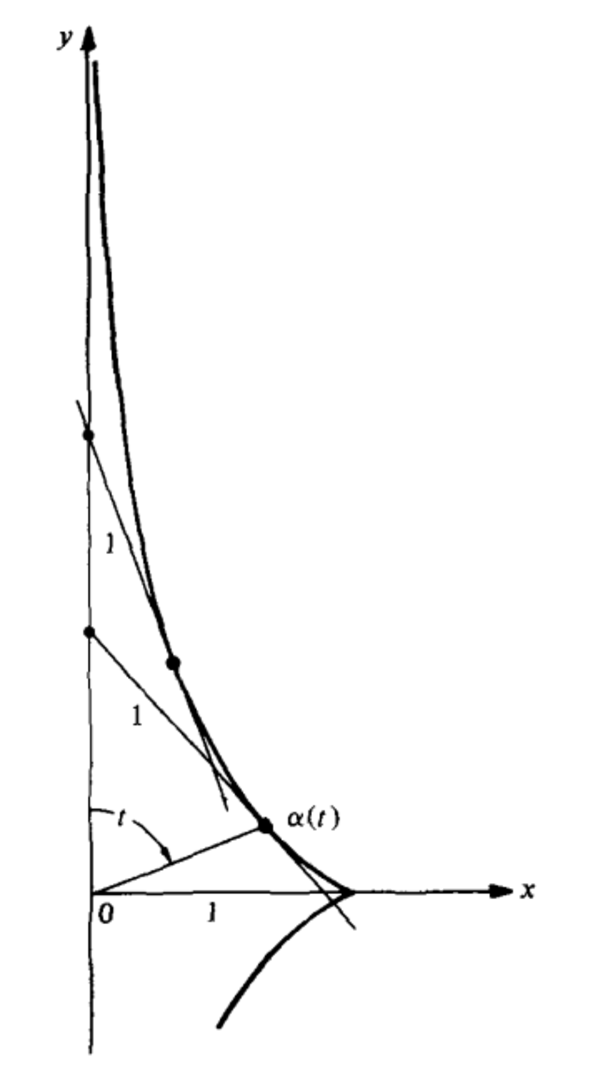
\includegraphics[scale=0.6]{1}
\caption{Mesh of the unit square with 4 triangles $\mathbb{P}_1$.}
\label{fig1}
\end{figure}
The tables \texttt{coords} and \texttt{triangles} define fully the mesh. However, it may be useful to use other tools. The following gives information on the edges of the mesh:
\begin{itemize}
\item \verb|edges|$\left(k,:\right) = $ numbers of the points that determine the edge numbered $k$,
\item \verb|edges_triangles|$\left\{ k \right\} =$ couples (element, local number of edge) for the elements which contain the edge number $k$. 
\end{itemize}
The following example precises the structure of this information: let us suppose that the edge numbered 2 is the edge that connects the points 2 and 5. Since it is shared by the elements 1 and 2, for which it is the edge respectively locally numbered 2 and 3, we have
\begin{verbatim}
edges(2,:) = [2,5]; edges_triangles{2} = {(1,2),(2,3)}.
\end{verbatim}
The computation with \textsc{Matlab} uses a \textit{cell-array}, which is more convenient than a table:
\begin{verbatim}
edges = [1,2;2,5;1,5;2,3;3,5;4,5;3,4;1,4];
edges_triangles{1} = [1,1];
edges_triangles{2} = [1,2;2,3];
edges_triangles{3} = [1,3;4,1];
edges_triangles{4} = [2,1];
edges_triangles{5} = [2,2;3,3];
edges_triangles{6} = [3,1;4,2];
edges_triangles{7} = [3,2];
edges_triangles{8} = [4,3];
\end{verbatim}

\begin{prob}\label{prob1.1}
Write a \textsc{Matlab} function which builds the tables \verb|edges| and \verb|edges_triangles|, the head of which is
\begin{verbatim}
function [edges, edges_triangle] = build_edge_connectivity(mesh)
\end{verbatim}
\end{prob}

\begin{proof}[Solution] 
To build the table \verb|edges|, we first initialize it as an `empty matrix'. We then loop on all the triangles of the given mesh. For each triangle, we compare\footnote{To compare easier, each edge of the considered triangle should be sorted first.} its three edges with all edges which is currently stored in the table \verb|edges|. There are only two possibilities. 
\begin{itemize}
\item The first possibility is that the considered edge has not been stored in the table \verb|edges| yet. In this case, we store that edge as a new row of the table \verb|edges|.
\item The second possibility is that the edge considered was stored in the table \verb|edges| already. In this case, we skip it and consider the next edge (or the next triangle in the loop, if all three edges of the current triangle have been considered).
\end{itemize}
After the table \verb|edges| is built successfully, we construct the table \verb|edges_triangles|. To do this, we loop on all the edges in the table \verb|edges|. For each edge, we make another loop on all the triangles of the mesh given. For each triangle in the second loop, we compare its three edges with the edge considered in the first loop. If there is a coincidence, we mark it on the current entry of the table \verb|edges_triangles| by the convention of local numbering of the reference triangle $\mathbb{P}_1$ described above.

Here is my \textsc{Matlab} script:
\begin{verbatim}
function [edges, edges_triangles] = build_edge_connectivity(mesh)
% Build the tables edges & edges_triangles of a mesh
% Author: Nguyen Quan Ba Hong
% Date: 06/10/2018
% Last Update: 16/10/2018
% Input:
% + mesh: a structured mesh
% Outputs:
% + edges: edges(K,:) = numbers of the points that determining the edge
% numbered K
% + edges_triangles{K} = couples(element, local number of edge) for the
% elements which contain the edge number K

%% Build Table edges
edges = [];
for K = 1:size(mesh.triangles,1) % Loop on Triangles of the Mesh
    % Read the Edges of the K-th Triangle
    temp = sort([mesh.triangles(K,[1,2]);
        mesh.triangles(K,[2,3]);
        mesh.triangles(K,[1,3])],2);
    flag = ones(3,1);
    for i = 1:3 % Loop on 3 Edges of the K-th Triangle
        for j = 1:size(edges,1)
            % Check if the edge considered is already in table edges or not
            if (edges(j,:) == temp(i,:))
                flag(i) = 0;
            end
        end
        if (flag(i) == 1)
            edges = [edges; temp(i,:)];
        end
    end
end

%% Build Cell-Array edges_triangles
for i = 1:size(edges,1) % Loop on the Edges
    edges_triangles{i} = [];
    for j = 1:size(mesh.triangles,1) % Loop on the Triangles of the Mesh
        if (edges(i,:) == sort(mesh.triangles(j,[1,2])))
            edges_triangles{i} = [edges_triangles{i}; j,1];
        elseif (edges(i,:) == sort(mesh.triangles(j,[2,3])))
            edges_triangles{i} = [edges_triangles{i}; j,2];
        elseif (edges(i,:) == sort(mesh.triangles(j,[1,3])))
            edges_triangles{i} = [edges_triangles{i}; j,3];
        end
    end
end
\end{verbatim}
For illustrations, running this script in the main function as
\begin{verbatim}
[edges,edges_triangles] = build_edge_connectivity(my_mesh);
for i = 1:size(edges,1)
   edges_triangles{i} 
end
\end{verbatim}
gives us exactly the \verb|edges| and \verb|edges_triangles| as above.
\end{proof}

\begin{prob}
Write a \textsc{Matlab} function the head of which is
\begin{verbatim}
function mesh_P2 = P1_to_P2(mesh_P1)
\end{verbatim}
and which builds a $\mathbb{P}_2$ mesh structure from a given $\mathbb{P}_1$ mesh structure. The local numbering should follow the convention of local numbering of the reference triangles $\mathbb{P}_2$ as follows: the midpoints of the edges 1, 2, 3 are labeled 4, 5, 6, respectively.
\end{prob}

\begin{proof}[Solution] 
To build a $\mathbb{P}_2$ mesh structure from a given $\mathbb{P}_1$ mesh structure, it suffices to modify the matrices \verb|coords| and \verb|triangles| of the old (i.e., $\mathbb{P}_1$) mesh structure.

The new \verb|coords| is modified easily by adding the midpoints of all edges of the $\mathbb{P}_1$ mesh. To do this, we first call the function \verb|build_edge_connectivity| of Problem \ref{prob1.1} to obtain the table \verb|edges|. Because the table \verb|edges_triangles| is not needed in this problem, so we replace this output with \verb|~| to save memory when the function \verb|build_edge_connectivity| is called, see the script below. We then loop on all edges of the $\mathbb{P}_1$ mesh structure\footnote{We should not loop on all triangles of the $\mathbb{P}_1$ mesh since all interior edges will be considered twice, and so are their midpoints.}. For each edge in the loop, we add its midpoint as a new row in the table \verb|coords|. An important notice is that the midpoint of the $i^{\rm th}$ edge in the $\mathbb{P}_1$ will be stored in the $\left(i+ \mbox{the number of nodes of }\mathbb{P}_1 \mbox{ mesh structure}\right)^{\rm th}$ row in the table \verb|coords| being updated. This notice is very useful in the below construction of the table \verb|triangles| for the new mesh structure.

The size of the table \verb|triangles| of the $\mathbb{P}_1$ mesh structure is $\mbox{the number of triangles of }\mathbb{P}_1 \times 3$, whereas the size of the table \verb|triangles| of the $\mathbb{P}_2$ mesh structure is $\mbox{the number of triangles of }\mathbb{P}_1 \times 6$. The last three columns, i.e., 4, 5, 6, are added to store the midpoints of three edges of each triangle of the $\mathbb{P}_1$ mesh structure.

Here is my \textsc{Matlab} script:
\begin{verbatim}
function mesh_P2 = P1_to_P2(mesh_P1)
% Build a P_2 mesh structure from a given P_1 mesh structure. The local
% numbering should follow the convention of Local numbering of the
% reference triangles P_2 as follows: the midpoints of the edges 1, 2, 3
% are labeled 4, 5, 6, respectively.
% Author: Nguyen Quan Ba Hong
% Date: 16/10/2018
% Last Update: 16/10/2018
% Input:
% + mesh_P1: a P_1-structured mesh
% Output:
% + mesh_P2: a P_2-structured mesh

%% Build edges & edges_triangles
[edges, ~] = build_edge_connectivity(mesh_P1);

%% Construct coords of mesh_P2
coords = mesh_P1.coords; % Utilize the Nodes of the Old Mesh
for i = 1:size(edges,1) % Loop on the Edges of mesh_P1
    % Add the Midpoint of i-th Edge of mesh_P1 to coords of mesh_P2
    coords = [coords; (coords(edges(i,1),:) + coords(edges(i,2),:))/2];
end

%% Construct Triangles of mesh_P2
triangles = zeros(size(mesh_P1.triangles,1),6);
triangles(:,[1,2,3]) = mesh_P1.triangles; % Utilize the Triangles of mesh_P1
for K = 1:size(mesh_P1.triangles,1) % Loop on Triangles of mesh_P1
    for i = 1:size(edges,1)
        if (sort(mesh_P1.triangles(K,[1,2])) == edges(i,:))
            triangles(K,4) = size(mesh_P1.coords,1) + i;
        elseif (sort(mesh_P1.triangles(K,[2,3])) == edges(i,:))
            triangles(K,5) = size(mesh_P1.coords,1) + i;
        elseif (sort(mesh_P1.triangles(K,[1,3])) == edges(i,:))
            triangles(K,6) = size(mesh_P1.coords,1) + i;
        end
    end
end

%% Build a P_2-Structured Mesh
mesh_P2 = mesh_new('Mesh_P2', coords, triangles);
\end{verbatim}
For illustrations, we run the following commands
\begin{verbatim}
mesh_P2 = P1_to_P2(my_mesh);
figure(1)
mesh_plot(mesh_P2,1)
\end{verbatim}
which produce the following figure
\begin{figure}[H]
\centering
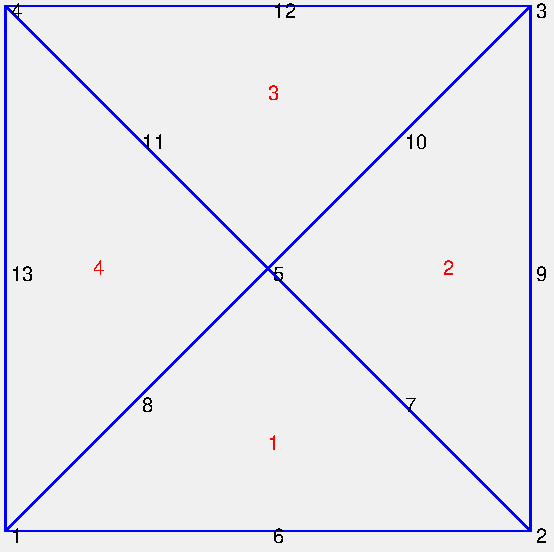
\includegraphics[scale=0.6]{Mesh_P2}
\caption{A $\mathbb{P}_2$ mesh structure.}
\end{figure}
This completes our solution.
\end{proof}
In the annex, we give the code of the function \verb|mesh_plot|, which offers a view of the mesh structure ($\mathbb{P}_1$ or $\mathbb{P}_2$).

\section{Triangulation of Delaunay}
The \textsc{Matlab} function \texttt{delaunay} builds a triangulation of Delaunay based on a set of points. If the table \texttt{coords}, of size $NbPoints \times 2$ contains the coordinates of the points of such a set, the call of the function is done with the following options
\begin{verbatim}
triangles = delaunay(coords(:,1),coords(:,2),{'Qt','Qbc','Qc','Qz'});
\end{verbatim}
However, when I run this command in my \textsc{Matlab} R2015a, the \textsc{Matlab}'s Command Window gives the following error
\begin{verbatim}
Error using delaunay
DELAUNAY no longer supports or requires Qhull-specific options.
 Please remove these options when calling DELAUNAY.
\end{verbatim}
And, the reduced command
\begin{verbatim}
triangles = delaunay(coords(:,1),coords(:,2));
\end{verbatim}
works well. So, we use this replacement to carry out the Delaunay's triangulation.

If the function is called with the table \texttt{coords} of the example of Fig. \ref{fig1}, one obtains the same triangulation with maybe different order in the numbering. Indeed,
\begin{figure}[H]
\centering
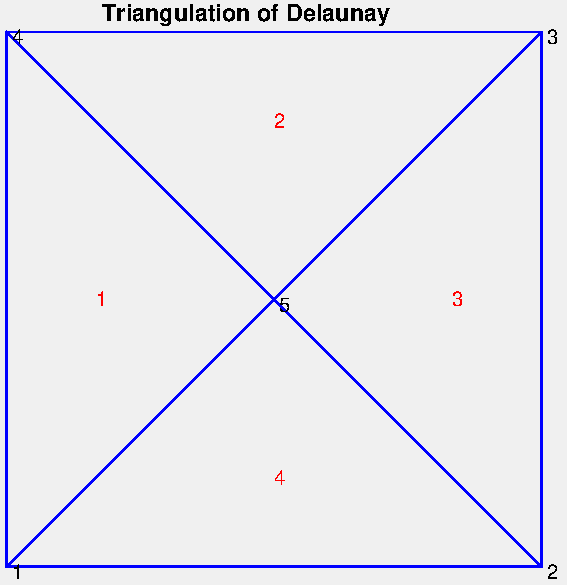
\includegraphics[scale=0.6]{8}
\caption{The triangulation of Delaunay has different orders in the numbering, Cf. Fig. \ref{fig1}.}
\label{fig8}
\end{figure}

\begin{prob}\label{prob2.1}
Write a \textsc{Matlab} function the head of which is
\begin{verbatim}
function [circumcenter, circumradius] = circumcircle(triangle_coor)
\end{verbatim}
and which computes the center of the circumscribed circle and its radius, for a triangle given through the coordinates of its vertices. The table \verb|triangle_coor| is of size $3\times 2$.

Using this function, plot the circumscribed circles of the triangles obtained with the function \verb|delaunay| and check that no open disk contains any point of the triangulation except the nodes of the mesh.
\end{prob}

\begin{proof}[Solution]
From the given coordinates of the vertices, we can easily compute the length of three edges and the area of that triangle. To compute the area $S$, there are two ways. The first one is to use the \textsc{Matlab} build-in function \verb|polyarea|. The second one is to use the Heron's formula
\begin{align}
S = \frac{1}{4}\left( {a + b + c} \right)\left( {b + c - a} \right)\left( {c + a - b} \right)\left( {a + b - c} \right).
\end{align}
To compute the radius of the circumscribed circle of the considered triangle, we use the formula
\begin{align}
R = \frac{{abc}}{{4S}}.
\end{align}
To compute the coordinates of the center of the circumscribed circle of the considered triangle, we use the following formula
\begin{align}
O = \frac{{{a^2}\left( {{b^2} + {c^2} - {a^2}} \right)A + {b^2}\left( {{c^2} + {a^2} - {b^2}} \right)B + {c^2}\left( {{a^2} + {b^2} - {c^2}} \right)C}}{{2\left( {{b^2}{c^2} + {c^2}{a^2} + {a^2}{b^2}} \right) - \left( {{a^4} + {b^4} + {c^4}} \right)}} , 
\end{align}
where $A$, $B$, and $C$ are the coordinates given, and $O$ denotes the coordinates of the center of the circumscribed circle of the triangle $ABC$.

Here is my \textsc{Matlab} script:
\begin{verbatim}
function [circumcenter, circumradius] = circumcircle(triangle_coor)
% Compute the center of the circumscribed circle and its radius, for a
% triangle given through the coordinates of its vertices
% Author: Nguyen Quan Ba Hong
% Date: 06/10/2018
% Last Update: 16/10/2018
% Input:
% + triangle_coor: is of size 3x2, gives the coordinates of three vertices
% of a triangle
% Outputs:
% + circumcenter: the center of the circumscribed circle of that triangle
% + circumradius: the radius of the circumscribed circle of that triangle

%% Compute Area of the Triangle
S = polyarea(triangle_coor(:,1), triangle_coor(:,2));

%% Compute Length of Edges of the Triangle
a = norm(triangle_coor(2,:) - triangle_coor(3,:)); % Length of edge BC
b = norm(triangle_coor(3,:) - triangle_coor(1,:)); % Length of edge CA
c = norm(triangle_coor(1,:) - triangle_coor(2,:)); % Length of edge AB

%% Alternative Way to Compute Area
% S = 1/4*sqrt((a+b+c)*(a+b-c)*(b+c-a)*(c+a-b)); % Heron's Formula

%% Compute Circumradius
circumradius = 1/4*a*b*c/S;

%% Compute Coordinates of Circumcenter
temp = [a^2*(b^2 + c^2 - a^2), b^2*(c^2 + a^2 - b^2), c^2*(a^2 + b^2 - c^2)];
circumcenter = temp(1)*triangle_coor(1,:) + temp(2)*triangle_coor(2,:) ...
    + temp(3)*triangle_coor(3,:);
circumcenter = circumcenter/sum(temp);
\end{verbatim}
Running following commands in the main script with the above meshes
\begin{verbatim}
my_mesh.name = 'Circumscribed Circles of Triangles';
figure
hold on
mesh_plot(my_mesh,0)
for i = 1:size(my_mesh.triangles,1)
    [center, radius] = circumcircle(my_mesh.coords(my_mesh.triangles(i,:),:));
    t = linspace(0,2*pi);
    x = center(1) + radius*cos(t);
    y = center(2) + radius*sin(t);
    plot(x,y);
end
axis equal
\end{verbatim}
gives us the following figure
\begin{figure}[H]
\centering
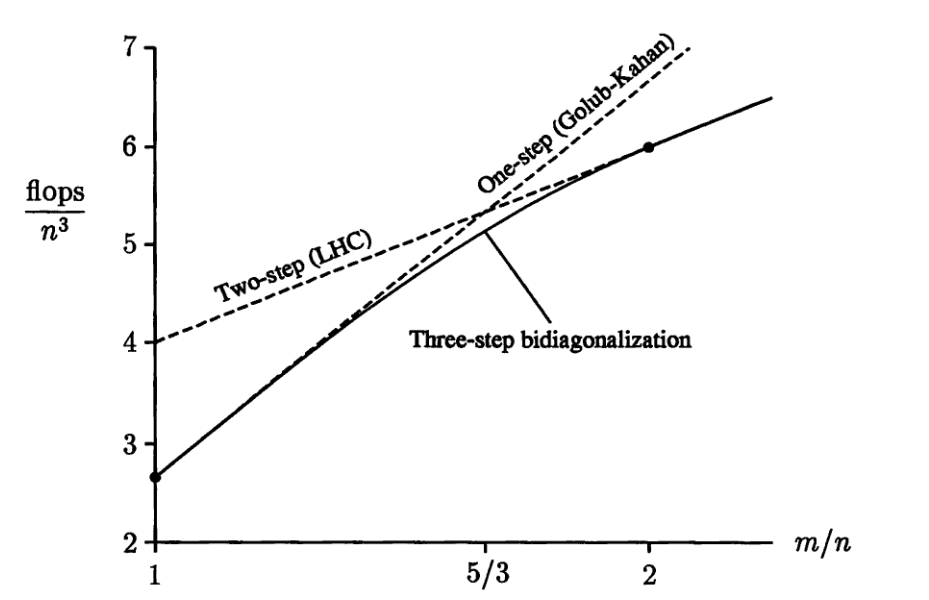
\includegraphics[scale=0.6]{9}
\caption{Circumscribed circles of the triangles obtained with the function \texttt{delaunay}.}
\label{fig9}
\end{figure}
It is clear that these circumscribed circles do not intersect any point of the triangulation except the nodes of the mesh.
\end{proof}

\begin{remark}
Here is an alternative \textsc{Matlab} script of Prof. \'Eric Darrigrand (see \emph{\cite{1}}):
\begin{verbatim}
function [circumcenter,circumradius] = circumcircle(triangle_coor)
% Compute the circumscribed circle data of a triangle given 
% by the coordinates of its vertices.
% Author: E.Darrigrand
% Date: 22/09/2011
% Last update: 22/09/2011
%
% usage: [circumcenter,circumradius] = circumcircle(triangle_coor)
%
% input -
%   triangle_coor : 3x2 array containing the coordinates of the vertices of the triangle.  
% output - 
%   circumcenter : center of the circumscribed circle
%   circumradius : radius of the circumscribed circle
%
a = triangle_coor(2,1) - triangle_coor(1,1);
b = triangle_coor(2,2) - triangle_coor(1,2);
c = triangle_coor(3,1) - triangle_coor(1,1);
d = triangle_coor(3,2) - triangle_coor(1,2);
e = 0.5 * (triangle_coor(2,1) + triangle_coor(1,1));
f = 0.5 * (triangle_coor(2,2) + triangle_coor(1,2));
g = 0.5 * (triangle_coor(3,1) + triangle_coor(1,1));
h = 0.5 * (triangle_coor(3,2) + triangle_coor(1,2));
%
alpha = a*e + b*f;
beta = c*g + d*h;
%
% With the notations above, the center has the coordinates (x,y) given below:
%
y = (alpha*c - a*beta)/(b*c - a*d);
if (abs(a)>abs(c))
   x = (alpha - b*y)/a;
else
   x = (beta - d*y)/c;
end
circumcenter = [x,y];
% 
% The radius is then the distance between the center and a vertex:
%
vect = [x,y]-triangle_coor(1,:);
circumradius = sqrt(vect*vect');
\end{verbatim}
\end{remark}

\section{Automatic Mesh}
If you have a triangulation from a set of points defined on the boundary of a domain of computation, to apply the finite elements you will require some points in the interior of the domain. The efficient methods are not easy to implement. Here, we consider a very simple way to implement a strategy that introduces points inside the domain of computation.

The principle is the following: we consider a triangulation $\mathcal{T}_n$ given at a step $n$. We determine the triangle $K\in \mathcal{T}_n$ which is identified as the ``worst'' (i.e., of greatest edge), and we denote $G$ its iso-barycenter. The new triangulation $\mathcal{T}_{n+1}$ is built by the insert of $G$ into the set of points of $\mathcal{T}_n$.

For the initialization of the process, we recommend the consideration of the triangulation $\mathcal{T}_0$ obtained from a subdivision of the polygonal boundary of the domain of computation. This subdivision would be a set of segments of size around $h$, where $h$ is the requested size for the elements of the mesh.

We mention again that this method is not efficient. Many different improvements can be done, for example, inserting the center of the circumscribed circle instead of its iso-barycenter (except if it is outside of the domain, in that case, we insert the midpoint of the largest edge).

\begin{prob}
Write a \textsc{Matlab} function which determines the ``worst'' element of a given mesh. Its head would be
\begin{verbatim}
function [triangle_number, max_edge_size] = find_worst_triangle(mesh)
\end{verbatim}
Then, write a function which builds the mesh according to the described strategy, from a subdivision of the boundary of the domain of computation:
\begin{verbatim}
function mesh_out = mesh_by_barycenters(boundary_vertices, mesh_size)
\end{verbatim}
They \verb|mesh_size| is a scalar which specify the required maximal size for the elements of the output mesh \verb|mesh_out|. The vector \verb|boundary_vertices| gives the coordinates of the vertices of the polygonal boundary of the computational domain.
\end{prob}

\begin{proof}[Solution]
Here is my \textsc{Matlab} script for the first task:
\begin{verbatim}
function [triangle_number, max_edge_size] = find_worst_triangle(mesh)
% Determine the "worst" element of a given mesh, i.e., the element has the 
% longest edge in the mesh, and provide the length of that longest edge
% Author: Nguyen Quan Ba Hong
% Date: 29/10/2018
% Last Update: 29/10/2018
% Input:
% + mesh: a mesh structure
% Outputs:
% + triangle_number: Index of the "worst" element of the mesh given
% + max_edge_size: the length of the longest edge in the mesh given

%% Utilize the Tables edges & edges_triangles
[edges, edges_triangles] = build_edge_connectivity(mesh);

%% Compute the Lengths of All Edges in the Mesh Given
length_edges = zeros(size(edges,1),1); 
for i = 1:size(edges,1) % Loop on All Edges of the Mesh Given
    % Compute the Length of the i-th Edge
    length_edges(i) = norm(mesh.coords(edges(i,1),:) - mesh.coords(edges(i,2),:));
end

%% Determine the Longest Edge and Its Index
[max_edge_size, edge_number] = max(length_edges);

%% Determine a Triangle Containing the Longest Edge
triangle_number = edges_triangles{edge_number}(1,1);
\end{verbatim}
And here is my \textsc{Matlab} script for the second task:
\begin{verbatim}
function mesh_out = mesh_by_barycenters(boundary_vertices, mesh_size)
% Build the mesh according to the following strategy:
% 1) For the initialization of the process: consider the triangulation
% T_0 obtained from a subdivision of the polygonal boundary of the domain
% of computation. This subdivison would be set of segments of size around
% mesh_size, where mesh_size is the requested size for the elements of the
% mesh.
% 2) Principle: Consider a triangulation T_n given at a step n, determine
% the "worst" triangle (i.e., of greatest edge), denote G its
% iso-barycenter. The new triangulation T_{n+1} is built by the insert of G
% into the set of points of T_n
% Author: Nguyen Quan Ba Hong
% Date: 08/10/2018
% Last Update: 29/10/2018
% Inputs:
% + boundary_vertices: vector which gives the coordinates of the
% vertices of the polygonal boundary of the computational domain
% + mesh_size: a scalar which specify the required maximal size for the
% elements of the output mesh
% Output:
% + mesh_out: the mesh built according to the described strategy, from a
% subdivision of the boundary of the domain of computation

%% Initialization of the Process: Zeroth Triangulation
coords = boundary_vertices; % Initialzie
for i = 1:size(boundary_vertices,1)-1 % Loop on All Non-Last Boundary Edges
    % Compute the Length of the i-th Boundary Edge
    length = norm(boundary_vertices(i,:) - boundary_vertices(i+1,:));
    loop = 2*ceil(length/mesh_size); % Number of Points for Partitioning
    for j = 1:loop-1
        % Equally-Spaced Partition of the i-the Boundary Edge
        coords = [coords; (loop-j)/loop*boundary_vertices(i,:) ...
            + j/loop*boundary_vertices(i+1,:)];
    end
end
% Compute the Length of the Last Boundary Edge
length = norm(boundary_vertices(i,:) - boundary_vertices(1,:));
loop = 2*ceil(length/mesh_size); % Number of Points for Partitioning
for j = 1:loop-1
    % Equally-Spaced Partition of the Last Boundary Edge
    coords = [coords; (loop-j)/loop*boundary_vertices(i,:) ...
        + j/loop*boundary_vertices(1,:)];
end

%% Perform Delaunay Triangulation of the New Table coords
triangles = delaunay(coords(:,1), coords(:,2));

%% Modify the Triangulation by Adding Iso-Barycenter
tol = 1e-2; % Tolerence for the criteria of degenerate triangles
while 1
    mesh_out = mesh_new('', coords, triangles); % Update Mesh Structure
    mesh_out = delete_degenerate_triangles(mesh_out, tol);
    % Find the Worst Element and Its Radius in the Current Mesh
    [triangle_number, max_edge_size] = find_worst_triangle(mesh_out);
    if (max_edge_size <= mesh_size)  % Stopping Criteria
        break % the Current Mesh Fulfills the Requirements on Size
    end
    % Add Iso-barycenter of the Worst Triangle to the Mesh
    coords = [coords; 1/3*sum(coords(mesh_out.triangles(triangle_number,:),:))];
    triangles = delaunay(coords(:,1), coords(:,2));
end
\end{verbatim}
This completes our solution.
\end{proof}






\section{Quality of the Mesh}
In the error estimates of the finite-element method, the \textit{roundness} of the elements of the mesh is significantly involved. It is given by the ratio between the radii of the circumscribed and inscribed circles:
\begin{align}
\sigma \left( K \right) := \frac{{h\left( K \right)}}{{\rho \left( K \right)}}.
\end{align}

\begin{prob}
Write a \textsc{Matlab} function which computes the roundness of a triangle. Its head would be
\begin{verbatim}
function sigma = roundness(triangle_coor)
\end{verbatim}
Then, write a function which computes the quality of a mesh, defined as the largest roundness of the elements:
\begin{verbatim}
function quality = mesh_quality(mesh)
\end{verbatim}
\end{prob}

\begin{proof}[Solution]
Here is my \textsc{Matlab} scripts:
\begin{verbatim}
function sigma = roundness(triangle_coor)
% Compute the roundness of a triangle, which is given by the ratio between
% the radii of the circumscribed and the inscribed circles
% Author: Nguyen Quan Ba Hong
% Date: 09/10/2018
% Last Update: 17/10/2018
% Input:
% + triangle_coor: is of size 3x2, gives the coordinates of three vertices
% of a triangle
% Output:
% + sigma: the roundness of the triangle given

%% Compute the Radius of the Circumscribed Circle of the Triangle 
[~, circumradius] = circumcircle(triangle_coor);

%% Compute the Radius of the Inscribed Circle of the Triangle
[~, inscribed_radius] = inscribed_circle(triangle_coor);

%% Compute the Roundness of the Triangle
sigma = circumradius/inscribed_radius;
\end{verbatim}
and
\begin{verbatim}
function quality = mesh_quality(mesh)
% Compute the quality of a given mesh, defined as the largest roundness of the
% elements of that mesh
% Author: Nguyen Quan Ba Hong
% Date: 09/10/2018
% Last Update: 17/10/2018
% Inpute:
% + mesh: a mesh structure
% Output:
% + quality: the quality of the mesh given

%% Store the Roundness of All Triangles in the Mesh
sigma = zeros(size(mesh.triangles,1),1);
for i = 1:size(mesh.triangles,1) % Loop on All Triangles of the Mesh
    % Compute the Roundness of i-th Triangle in the Mesh
    sigma(i) = roundness(mesh.coords(mesh.triangles(i,:),:)); 
end

%% Compute the Quality of the Given Mesh
quality = max(sigma);
\end{verbatim}
This completes our solution.
\end{proof}
Numerous strategies exist to improve the quality of a given mesh. Here, we propose to implement the most accessible: each interior point of the mesh (i.e., not on the boundary) is replaced by the iso-barycenter of its neighbors.

\begin{prob}
Write a \textsc{Matlab} function which optimizes a mesh following the method described just above:
\begin{verbatim}
function mesh_out = mesh_optimize(mesh_in)
\end{verbatim}
(you may need a function which determines if a point is interior or not; you may use the list \verb|edges_triangles| built in Problem \ref{prob1.1}).
\end{prob}

\begin{proof}[Solution]
\begin{verbatim}
function mesh_out = mesh_optimize(mesh_in)
% Optimize a mesh by the following strategy: Each interior point of the
% mesh (i.e. not on the boundary) is replaced by the iso-barycenter of its
% neighbors
% Author: Nguyen Quan Ba Hong
% Date: 08/10/2018
% Last Update: 17/10/2018
% Input:
% + mesh_in: a mesh structure needing improving the quality
% Output: 
% + mesh_out: optimized mesh structure

%% Reuse All the Nodes on the Boundary of the Mesh Given
boundary_nodes = boundarynodes(mesh_in); % Initialize
coords = boundary_nodes; % Storage of Nodes of the New Mesh

%% Add Iso-Barycenters of All Triangles of the Mesh Given
for i = 1:size(mesh_in.triangles,1) % Loop on All Triangles of the Mesh Given
    coords = [coords; 1/3*sum(mesh_in.coords(mesh_in.triangles(i,:),:))];
end

%% Create the Final Mesh
triangles = delaunay(coords(:,1), coords(:,2)); % Delaunay Triangulation
mesh = mesh_new('', coords, triangles);
mesh_out = delete_degenerate_triangles(mesh, 1e-2); 
\end{verbatim}
\end{proof}


\section{Appendices: \textsc{Matlab} Scripts}

 

\subsection{Delete All Degenerate Triangles in a Mesh}
\begin{verbatim}
function mesh_out = delete_degenerate_triangles(mesh, tol)
% Delete all degenerate triangles in the mesh given. Define a "degenerate"
% triangle as a triangle whose the radius of its corresponding inscribed
% circle is less than some given tolerance, e.g. inscribed_radius < 1e-3
% Author: Nguyen Quan Ba Hong
% Date: 08/10/2018
% Last Update: 29/10/2018
% Input:
% + mesh: a mesh structure
% Output:
% + mesh_out: a mesh structure without degenerate triangles 

%% Classify Degenerate and Nondegenerate Triangles
triangles = []; % Initialize
for i = 1:size(mesh.triangles,1) % Loop on All Triangles of the Mesh Given
    % Compute the Inscribed Radius of the i-th Triangle
    [~, inscribed_radius] = inscribed_circle(mesh.coords(mesh.triangles(i,:),:));
    if (inscribed_radius > tol) 
         triangles = [triangles; mesh.triangles(i,:)];
    end
end

%% Create a New Mesh without Degenerate Triangles
mesh_out = mesh_new('', mesh.coords, triangles);
\end{verbatim}
\subsection{Mesh Improvement}

\subsection{Mesh Refinement}
Here is my script:
\begin{verbatim}
function mesh_P2 = P1_to_P2(mesh_P1)
% Refine a mesh
% Author: Nguyen Quan Ba Hong
% Date: 06/10/2018
% Last Update: 08/10/2018

[edges,edges_triangles] = build_edge_connectivity(mesh_P1);

%% Construct coords of mesh_P2
coords = mesh_P1.coords; % Utilize the nodes of the old mesh
for i = 1:size(edges,1)
    % Add the midpoint of i-th edge of mesh_P1
    coords = [coords;(coords(edges(i,1),:) + coords(edges(i,2),:))/2];
end

%% Construct triangles of mesh_P2
triangles = []; % Initialize triangles of mesh_P2
for i = 1:size(mesh_P1.triangles,1)
    for j = 1:size(edges,1)
        if (edges(j,:) == sort([mesh_P1.triangles(i,1),mesh_P1.triangles(i,2)]))
            midpoint_edge1 = j + size(mesh_P1.coords,1);
        end
        if (edges(j,:) == sort([mesh_P1.triangles(i,2),mesh_P1.triangles(i,3)]))
            midpoint_edge2 = j + size(mesh_P1.coords,1);
        end
        if (edges(j,:) == sort([mesh_P1.triangles(i,1),mesh_P1.triangles(i,3)]))
            midpoint_edge3 = j + size(mesh_P1.coords,1);
        end
    end
    triangles = [triangles;mesh_P1.triangles(i,1),midpoint_edge1,midpoint_edge3;
        mesh_P1.triangles(i,2),midpoint_edge2,midpoint_edge1;
        mesh_P1.triangles(i,3),midpoint_edge3,midpoint_edge2;
        midpoint_edge1,midpoint_edge2,midpoint_edge3];
end
mesh_P2 = mesh_new('Mesh',coords,triangles);
\end{verbatim}
To implement how this subscript works, we run the following commands in the main script
\begin{verbatim}
for i = 1:5
    my_mesh = P1_to_P2(my_mesh);
    figure(i)
    mesh_plot(my_mesh,0)
    axis equal
end
\end{verbatim}
to obtain
\begin{figure}[H]
\centering
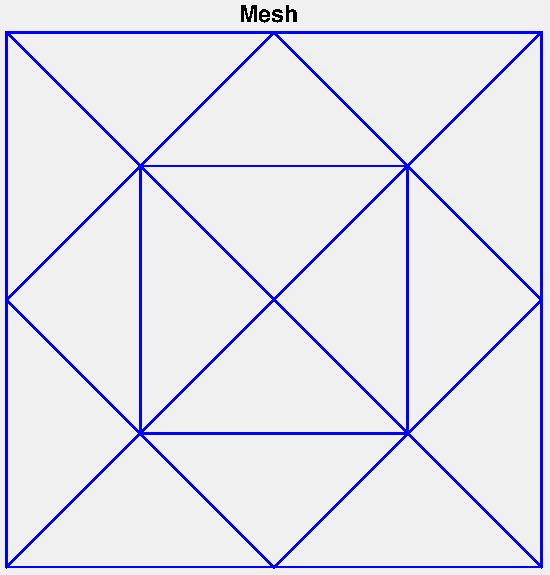
\includegraphics[scale=0.6]{2}
\caption{Apply the script \texttt{P1\_to\_P2} once without showing numbers.}
\label{fig2}
\end{figure}

\begin{figure}[H]
\centering
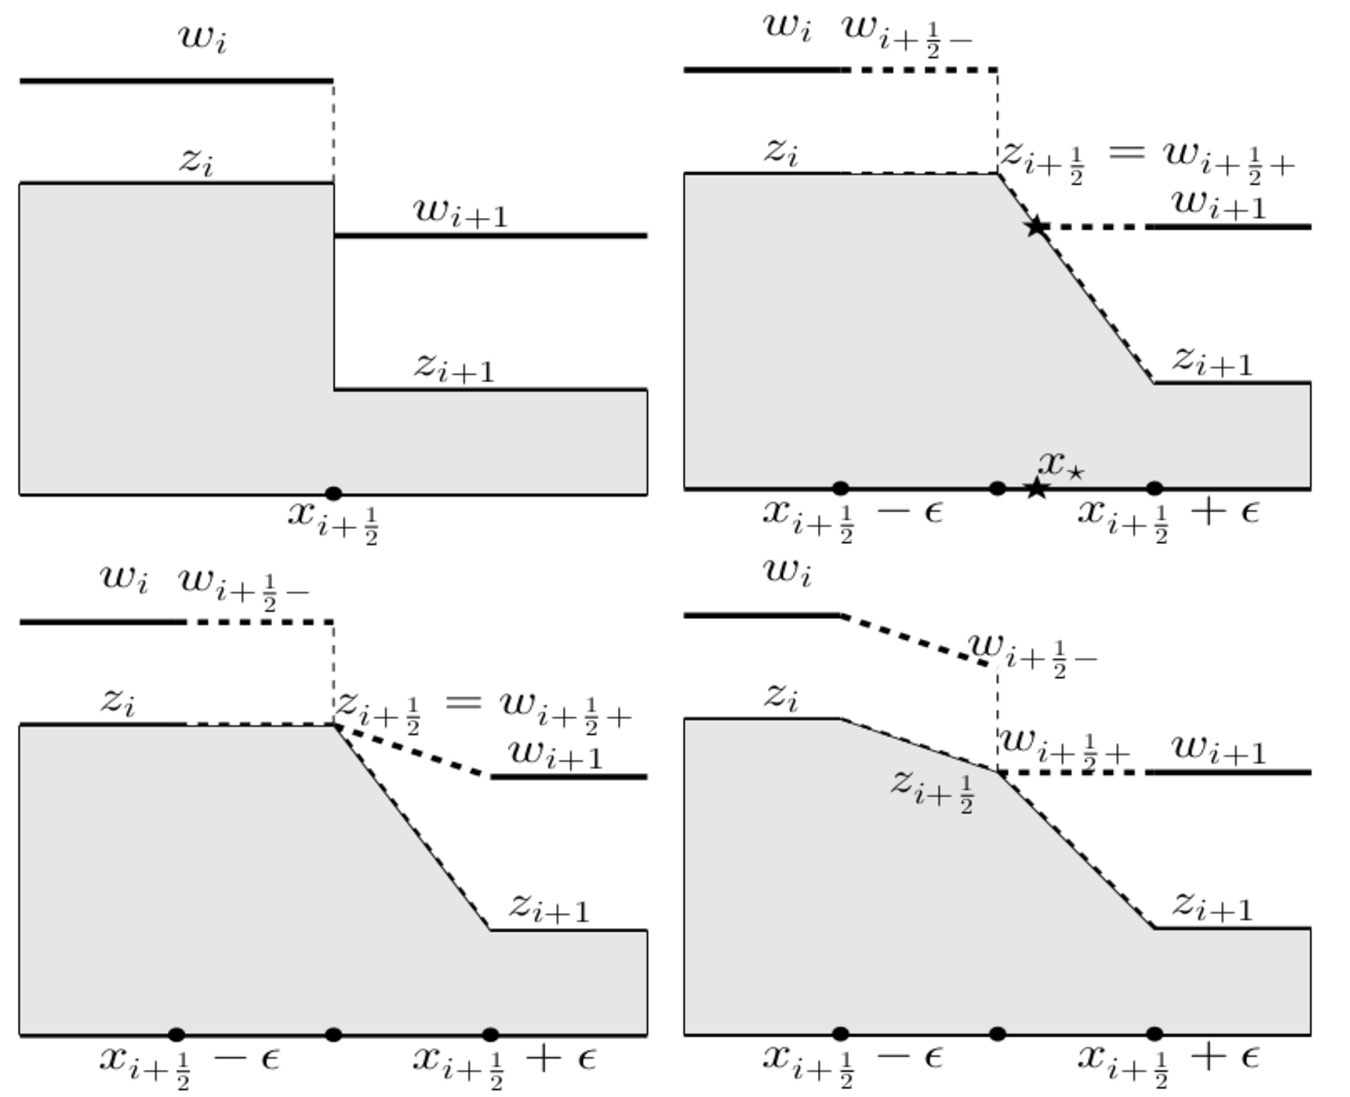
\includegraphics[scale=0.6]{3}
\caption{Apply the script \texttt{P1\_to\_P2} twice without showing numbers.}
\label{fig3}
\end{figure}

\begin{figure}[H]
\centering
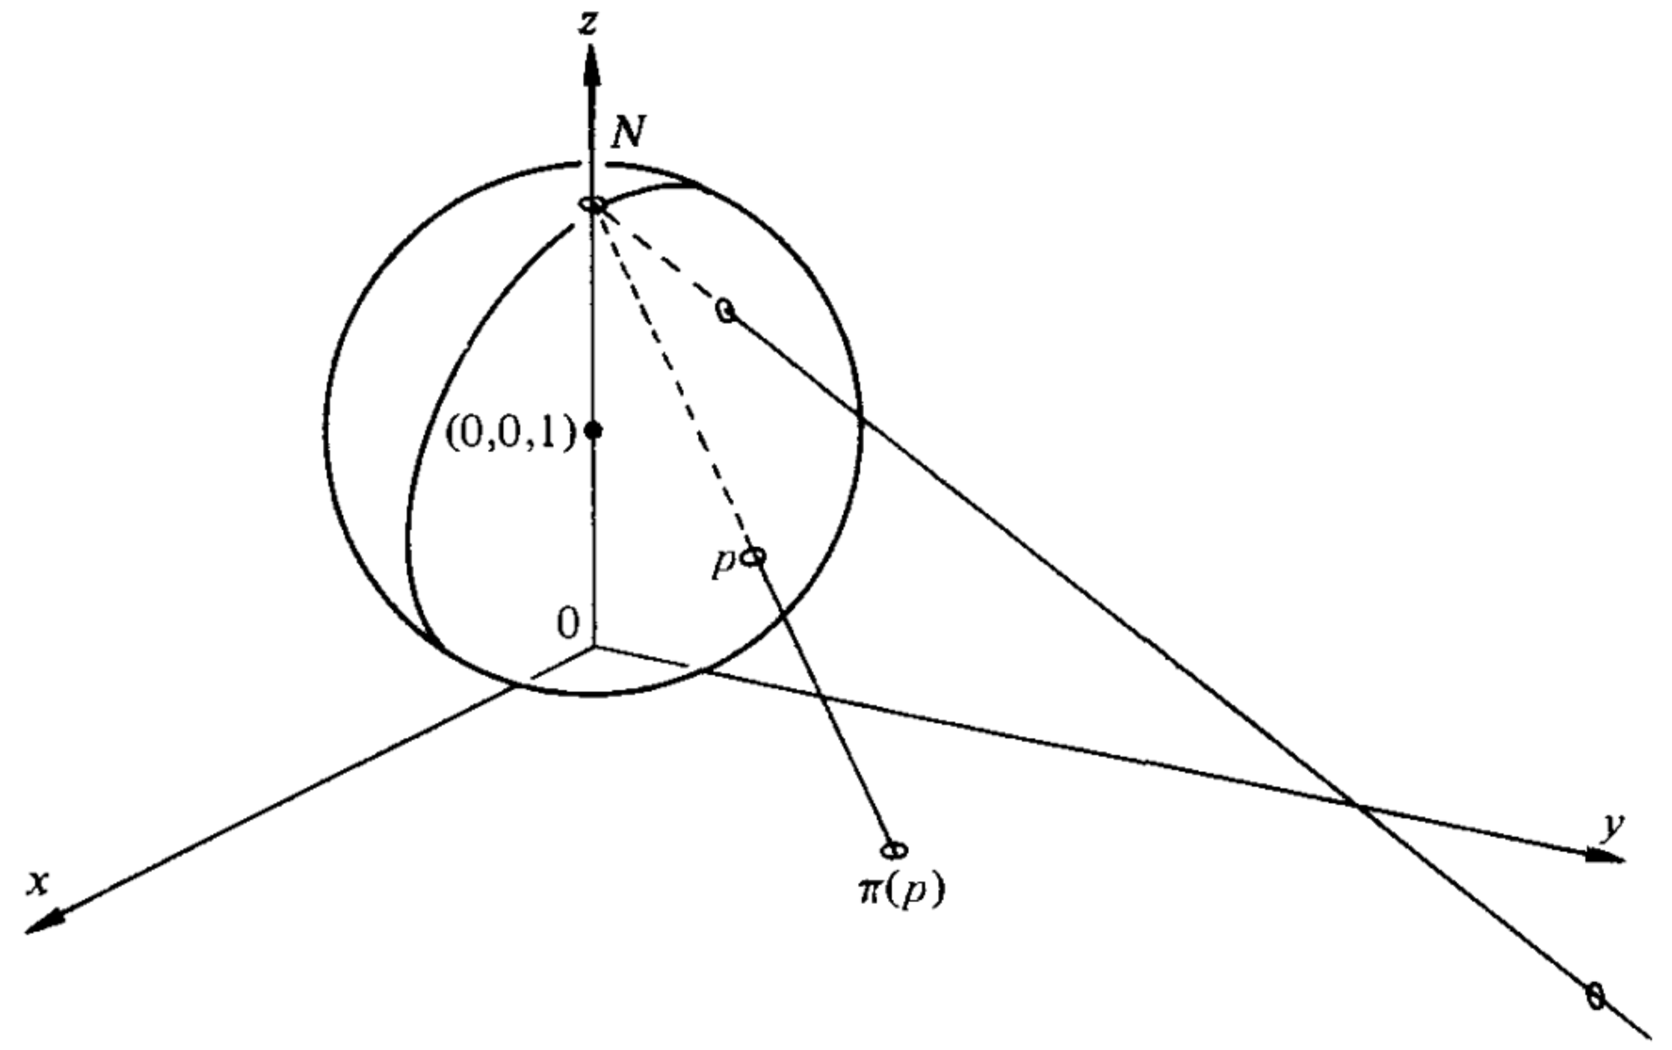
\includegraphics[scale=0.6]{4}
\caption{Apply the script \texttt{P1\_to\_P2} three times without showing numbers.}
\label{fig4}
\end{figure}

\begin{figure}[H]
\centering
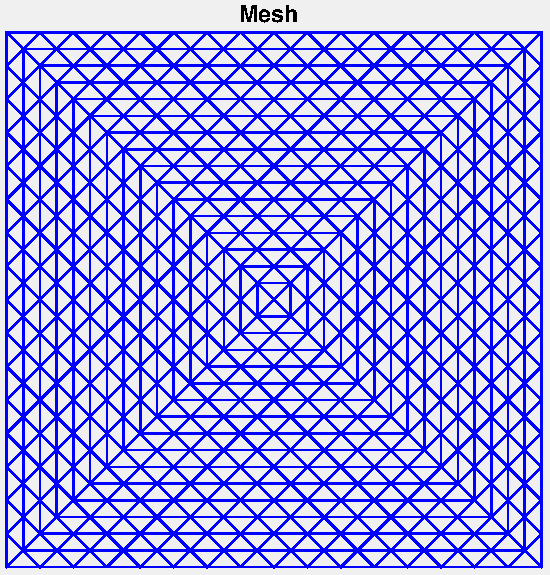
\includegraphics[scale=0.6]{5}
\caption{Apply the script \texttt{P1\_to\_P2} four times without showing numbers.}
\label{fig5}
\end{figure}
and with the command \verb|mesh_plot(my_mesh,1)|,
\begin{figure}[H]
\centering
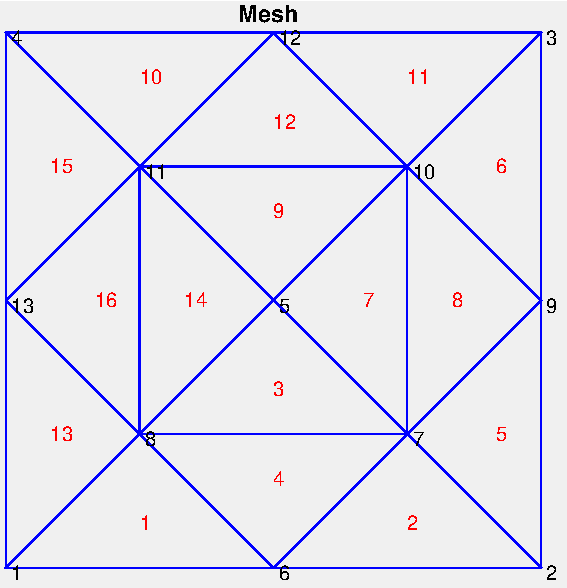
\includegraphics[scale=0.6]{6}
\caption{Apply the script \texttt{P1\_to\_P2} four times with showing numbers.}
\label{fig6}
\end{figure}

\begin{figure}[H]
\centering
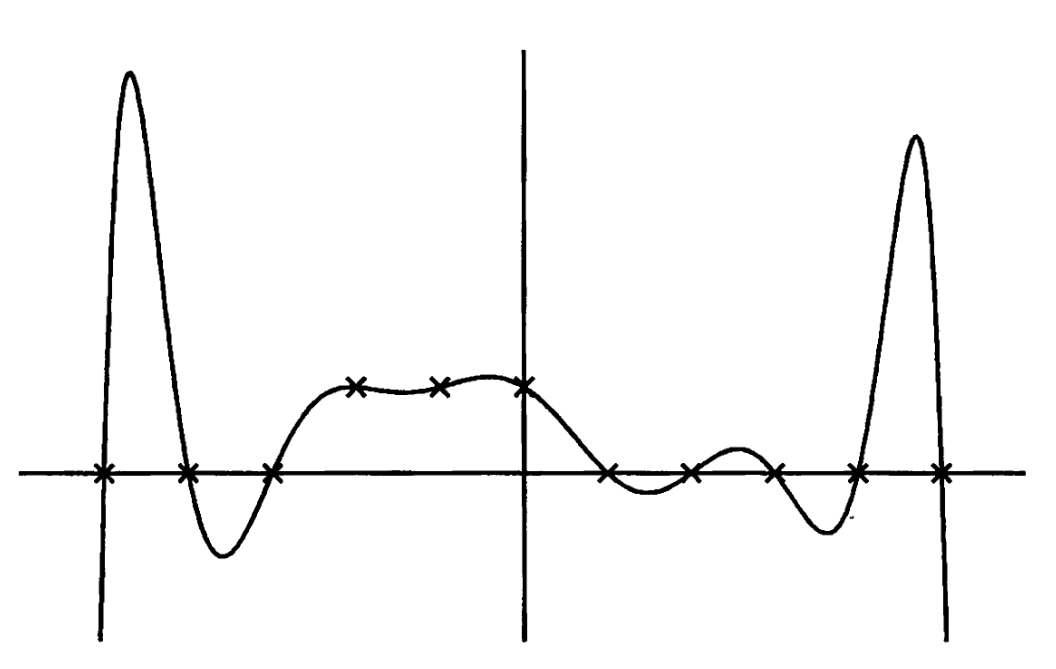
\includegraphics[scale=0.6]{7}
\caption{Apply the script \texttt{P1\_to\_P2} four times with showing numbers.}
\label{fig7}
\end{figure}

\begin{figure}[H]
\centering
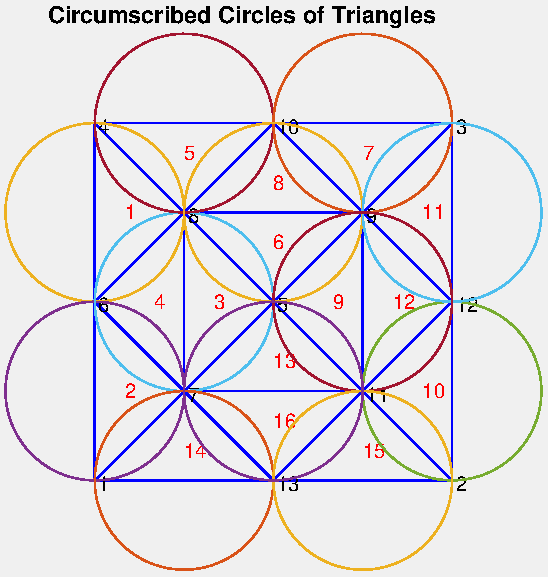
\includegraphics[scale=0.6]{10}
\caption{Circumscribed circles of the triangles obtained with the function \texttt{delaunay}.}
\label{fig10}
\end{figure}

\begin{figure}[H]
\centering
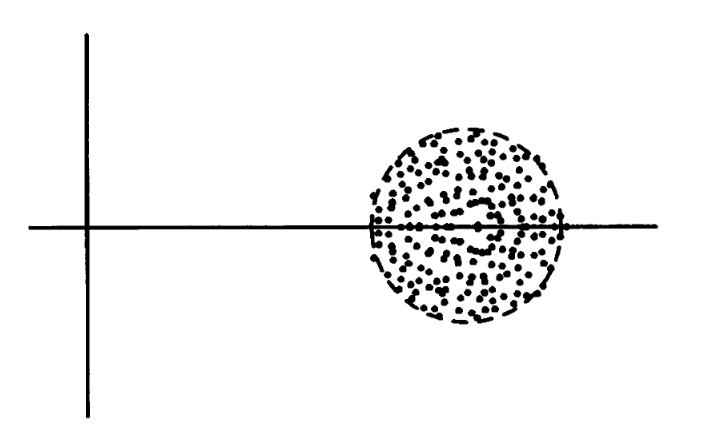
\includegraphics[scale=0.6]{11}
\caption{Circumscribed circles of the triangles obtained with the function \texttt{delaunay}.}
\label{fig11}
\end{figure}

\begin{figure}[H]
\centering
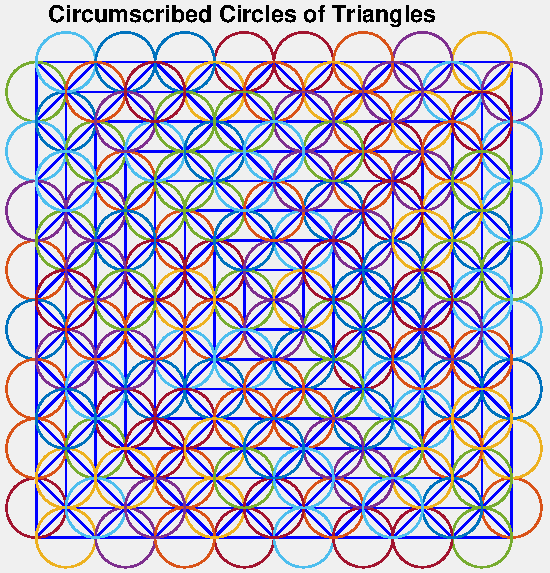
\includegraphics[scale=0.6]{12}
\caption{Circumscribed circles of the triangles obtained with the function \texttt{delaunay}.}
\label{fig12}
\end{figure}

\begin{figure}[H]
\centering
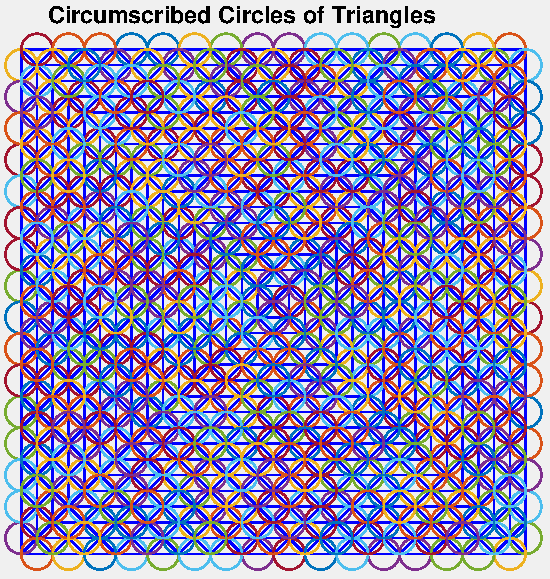
\includegraphics[scale=0.6]{13}
\caption{Circumscribed circles of the triangles obtained with the function \texttt{delaunay}.}
\label{fig13}
\end{figure}


\begin{proof}[Solution]
First we need to compute the center of the inscribed circle and its radius. This task is similar to the one in Problem \ref{prob2.1}. With the same notations $a$, $b$, $c$, $S$ before, the following formulas are used 
\begin{align}
r &= \frac{{2S}}{{a + b + c}},\\
I &= \frac{{aA + bB + cC}}{{a + b + c}}.
\end{align}
Here is my \textsc{Matlab} script for computing the center and radius of the inscribed circle of a triangle in terms of the coordinates of its vertices.
\begin{verbatim}
function [inscribed_center, inscribed_radius] = inscribed_circle(triangle_coor)
% Compute the center & the radius of the inscribed circle of a triangle whose
% coordinates of its vertices are given
% Author: Nguyen Quan Ba Hong
% Date: 09/10/2018
% Last Update: 17/10/2018
% Input:
% + triangle_coor: is of size 3x2, gives the coordinates of three vertices
% of a triangle
% Outputs:
% + inscribed_center: the center of the inscribed circle of that triangle
% + inscribed_radius: the radius of the inscribed circle of that triangle

%% Compute the Area of the Triangle
S = polyarea(triangle_coor(:,1), triangle_coor(:,2));

%% Compute the Length of Edges of the Triangle
a = norm(triangle_coor(2,:) - triangle_coor(3,:)); % Length of edge BC
b = norm(triangle_coor(3,:) - triangle_coor(1,:)); % Length of edge CA
c = norm(triangle_coor(1,:) - triangle_coor(2,:)); % Length of edge AB

%% Alternative Way to Compute Area of the Triangle
% S = 1/4*sqrt((a+b+c)*(a+b-c)*(b+c-a)*(c+a-b)); % Heron's formula

%% Compute Inscribed Radius of the Triangle
inscribed_radius = 2*S/(a+b+c);

%% Compute Coordinates of Circumcenter
inscribed_center = 1/(a+b+c)*(a*triangle_coor(1,:) + b*triangle_coor(2,:) ...
    + c*triangle_coor(3,:));
\end{verbatim}
Here is my script for the first part:
\begin{verbatim}
function [triangle_number, max_radius] = find_worst_triangle(mesh)
% Determine the "worst" element of a given mesh, i.e., the element of
% greatest inscribed radius, & that greast value
% Author: Nguyen Quan Ba Hong
% Date: 08/10/2018
% Last Update: 17/10/2018
% Input:
% + mesh: a mesh structure
% Outputs:
% + triangle_number: Index of the "worst" element of the given mesh
% + max_radius: the maximum of the radius of the inscribed circle of the
% triangles of the given mesh

radius = zeros(size(mesh.triangles,1),1);
for i = 1:size(mesh.triangles,1)
    % Compute Inscribed Radius of the i-th Triangle in the Mesh
    [~, inscribed_radius] = inscribed_circle(mesh.coords(mesh.triangles(i,:),:));
    radius(i) = inscribed_radius;
end
% Determine the maximal radius and the index of the "worst" triangle
[max_radius, triangle_number] = max(radius);
\end{verbatim}
and that for the second part:
\begin{verbatim}
function mesh_out = mesh_by_barycenters(boundary_vertices, mesh_size)
% Build the mesh according to the following strategy:
% 1) For the % initialization of the process: consider the triangulation
% T_0 obtained % from a subdivision of the polygonal boundary of the domain
% of computation. This subdivison would be set of segments of size around
% mesh_size, where mesh_size is the requested size for the elements of the
% mesh.
% 2) Principle: Consider a triangulation T_n given at a step n, determine
% the "worst" triangle (i.e., of greatest inscribed radius), denote G its
% iso-barycenter. The new triangulation T_{n+1} is built by the insert of G
% into the set of points of T_n
% Author: Nguyen Quan Ba Hong
% Date: 08/10/2018
% Last Update: 17/10/2018
% Inputs:
% + boundary_vertices: vector which gives the coordinates of the
% vertices of the polygonal boundary of the computational domain
% + mesh_size: a scalar which specify the required maximal size for the
% elements of the output mesh
% Output:
% + mesh_out: the mesh built according to the described strategy, from a
% subdivision of the boundary of the domain of computation

%% Initialization of the Process: Zeroth Triangulation
coords = [];
% Index the Vertices of Polygonal Boundary, the first vertex is also
% counted again in the last edge, but with the largest numbering
index_boundary_vertices = ones(size(boundary_vertices,1) + 1,1);
for i = 1:size(boundary_vertices,1) % Loop on All Boundary Edges
    % Add Coordinate of the i-th Vertex of Polygonal Boundary to coords
    coords = [coords; boundary_vertices(i,:)];
    if (i < size(boundary_vertices,1)) % Not the Last Boundary Edge
        % Compute the Length of the i-th Boundary Edge
        length = norm(boundary_vertices(i,:) - boundary_vertices(i+1,:));
        loop = ceil(length/mesh_size); % Number of Points for Partitioning
        for j = 1:loop-1
            % Equally-Spaced Partition of the i-the Boundary Edge
            coords = [coords; (loop-j)/loop*boundary_vertices(i,:) ...
                + j/loop*boundary_vertices(i+1,:)];
        end
    else % The Last Edge in the Polygonal Boundary
        % Compute the Length of the Last Boundary Edge
        length = norm(boundary_vertices(i,:) - boundary_vertices(1,:));
        loop = ceil(length/mesh_size); % Number of Points for Partitioning
        for j = 1:loop-1
            % Equally-Spaced Partition of the Last Boundary Edge
            coords = [coords; (loop-j)/loop*boundary_vertices(i,:) ...
                + j/loop*boundary_vertices(1,:)];
        end
    end
    % Index the (i+1)-th Vertices of the Boundary
    index_boundary_vertices(i+1) = index_boundary_vertices(i) + loop;
end
triangles = delaunay(coords(:,1), coords(:,2));

%% Delete Degenerate Triangles in Delaunay Triangualation
new = []; % Goal: New Triangles Storage without Degenerate Triangles
for i = 1:size(triangles,1)
    flag = 1; % Boolean Variable for Checking Degeneracy of Triangles
    for j = 1:size(boundary_vertices,1) % Loop on All Boundary Edges
        temp = sort(triangles(i,:),2);
        % For the Last Edge of Boundary
        % Condition for Degeneracy of the Triangle on the Last Boundary Edge
        if (temp (1) == 1 && index_boundary_vertices(size(boundary_vertices,1))...
                <= temp(2))
            flag = 0; % Detect Degeneracy
        end
        % For the Non-Last Edge of Boundary
        % Condition for Degeneracy of the Triangle on the Non-Last Boundary Edge
        if ((index_boundary_vertices(j) <= temp(1)) && (temp(3) ...
                <= index_boundary_vertices(j+1)))
            flag = 0; % Detect Degeneracy
        end
    end
    if (flag == 1) % The Considered Triangle is Not Degenerate
        new = [new; triangles(i,:)]; % Store this Non-Degenerate Triangle
    end
end
triangles = new; % Updated triangles without Degenerate Elements

%% Modify the Triangulation by Adding Iso-Barycenter
while 1
    mesh_out = mesh_new('',coords,triangles); % Update Mesh Structure
    % Find the Worst Element and Its Radius in the Current Mesh
    [triangle_number, max_radius] = find_worst_triangle(mesh_out);
    % Stopping Criteria
    if (max_radius <= mesh_size)
        break % the Current Mesh Fulfills the Requirements
    end
    % Add Iso-barycenter of the Worst Triangle to the Mesh
    coords = [coords; 1/3*sum(coords(triangles(triangle_number,:),:))];
    % Update New Three Triangles Generated by Inserting the Iso-Barycenter
    triangles = [triangles; triangles(triangle_number,[1 2]), size(coords,1);
        triangles(triangle_number,[2 3]), size(coords,1);
        triangles(triangle_number,[3 1]), size(coords,1)];
    triangles(triangle_number,:) = []; % Delete the Worst Triangle
end

%% Create Final Mesh
mesh_out = mesh_new('',coords,triangles);
\end{verbatim}
This completes our solution.
\end{proof}
%\section*{Appendix A. Supplementary notes}



%\section*{Acknowledgment}

\begin{thebibliography}{999}
\bibitem {1} \url{https://perso.univ-rennes1.fr/eric.darrigrand-lacarrieu/Teaching/M2RFEorganisation.html}
\end{thebibliography}
%\bibliographystyle{siam}
%\bibliography{MYBIB}
%\Addresses
\end{document}